% reducesymm/QFT/worldline.tex
%%%%%%%%%%%%%%%%%%%%%%%%%%%%%%%%%%%%%%%%%%%%%%%%%%%%%%%%%%%%%%%%%%%%%%%%%

\section{Worldline formalism}
\label{sect:worldline}

How and why Feynman in 1950 introduced `worldline formalism' (initially
for scalar QED, appendix to \refref{Feynman50}, then for spinor QED,
appendix to \refref{Feynman51}) is explained in Schubert 2001
report\rf{Schubert01} (which also has an extensive bibliography up to
2001).
In 1982 Affleck, Alvarez, and Manton\rf{AffAlMa82} used the Feynman
worldline path integral representation of the quenched effective action
for scalar QED in the constant electric field.

For the remainder of this section we shall consider only the quenched
QED, \ie, restrict our considerations only to sets of diagrams with no
lepton loop insertions.

A formula for the charged scalar propagator to emit and reabsorb $N$
photons as it propagates from $x'$ to $x$ can be derived
as follows\rf{AhBaSc16}.
The free scalar propagator for the Euclidean
Klein-Gordon equation\rf{Schubert12,AhBaSc16} is
\beq
D_0(x,x')=\bra{x}\frac{1}{-\Box +m^2}\ket{x'}
\,,
\ee{Schubert12(1.1)}
where $\Box$ is the $D$-dimensional Laplacian. Exponentiate the
denominator following Schwinger,
% proper-time parameter $T$
\beq
D_0(x,x')=\int_0^\infty\!\!dT\,{e}^{-m^2T}\bra{x}e^{-T(-\Box)}\ket{x'}
\,,
\ee{Schubert12(1.4)}
Replace the operator in the exponent by a path integral
\beq
D_0(x,x')=\int_0^\infty\!\!dT\,e^{-m^2T}
\int_{x(0)=x'}^{x(T)=x}\!\!\!\!\mathcal{D}x(\tau)\,
    e^{-\int_0^T\!\!d\tau \frac{1}{4}\dot{x}^2}
\,,
\ee{Schubert12(1.7)}
where $\tau$ is a proper-time parameter (the fifth parameter\rf{Fock37}), and
the dot denotes a derivative with respect to the proper time. This is the
\emph{worldline path integral} representation of the relativistic propagator
of a scalar particle in Euclidean space-time. In the vacuum (no background
field), it is easily evaluated by standard methods and leads to the usual
space and momentum space free propagators,
    \PC{2017-06-17
Here a study of Sect.~6. {\em Worldline formalism} of Gelis and N.
Tanji\rf{GelTan16} might be helpful - it reexpresses the integral as an
average over Wilson loops.
    }
\beq
\int_{x(0)=x'}^{x(T)=x}\!\!\!\!\mathcal{D}x(\tau)\,
    e^{-\int_0^T\!\!d\tau \frac{1}{4}\dot{x}^2}
        =
\frac{1}{(4\pi T)^{d/2}}
\,.
\ee{GelTan16(186)}
Adding the QED
interaction terms leads to the Feynman's worldline path integral
representation\rf{Feynman50} of the charged scalar propagator  of mass
$m$ in the presence of a background field $A(x)$,
\beq
D(x,x')=\int_0^\infty\!\!dT\,e^{-m^2T}
    \int_{x(0)=x'}^{x(T)=x}\!\!\mathcal{D}x(\tau)\,
            {e}^{-S_0-S_e-S_i}
\,,
\ee{AhBaSc16(1)}
where the suffix (0) indicates the free propagation
\beq
S_0 = \int_0^T\!\!d\tau \frac{1}{4}\dot{x}^2
\,,
\ee{Ahmadiniaz1}
(e) is the interaction of the charged scalar with the external field
\beq
S_e = -ie\int_0^T\!\!d\tau\,\dot{x}^\mu A_\mu(x(\tau))
\,,
\ee{Ahmadiniaz2}
and (i) are the virtual photons exchanged along the charged particle's
trajectory
\beq
S_i = \frac{e^2}{2}\int_0^T\!\!d\tau_1\int_0^T\!\!d\tau_2\,
      \dot{x}_1^\mu\,D_{\mu\nu}(x_1-x_2)\,\dot{x}_2^\nu
\,,
\ee{Ahmadiniaz3}
where $D_{\mu\nu} $ is the $x$-space photon propagator.
% In $D$ dimensions and arbitrary covariant gauge

The formula \refeq{AhBaSc16(1)} involves
(i) a path integral over all the worldlines $x(\tau')$, \ie, closed paths in
Euclidean space-time parameterized by the proper time $\tau'\in[0,\tau]$, and
(ii) an ordinary integral over the length $\tau$ of these paths.
The sum over all the worldlines accounts for the quantum fluctuations in
space-time, and the prefactor $\exp(-m^2T)$ suppresses the very long
worldlines that explore regions of space-time much larger than the Compton
wavelength of the particles. The ultraviolet properties of the theory are
encoded in the short worldlines limit $\tau\to{0}$. The
Euclidean space-time guarantees that both types of integrals are convergent.

Consider next the charged scalar field in external field, neglecting
internal photon loops. By taking the constant external field $A(x)$ to be
a sum of $N$ plane waves, one obtains the rule for inserting $N$ external
photons:
\bea
D_{(N)}(x,x')
%\langle 0|T \phi (x) \phi (y) |0\rangle_{(N)}
&=& (-\lambda)^N
 \int_0^\infty \! dT \,e^{-m^2 T}
 \int_0^Td\tau_1 \cdots \int_0^Td\tau_N
 \nonumber\\ &&
\times  \int_{_{x(0)=y}}^{^{\, x(T)=x}}
\!\!\!\!\!\!\!\!\!\!\!\! {\cal D}x
\,e^{i\sum_{i=1}^Nk_i\cdot x(\tau_i)}
e^{ -\int_0^Td\tau\, {1\over 4} \dot x^2}
\,.
\label{Nprop}
\eea
For the spinor case, the magnetic moment will be given by the term linear
in a constant external field $A(x)$, and in order to define gauge sets,
one will have to distinguish the in- and out-electron lines.

The object of great interest to us is the quenched internal virtual
photons term \refeq{Ahmadiniaz3}:
\beq
\int_{x(0)=x'}^{x(T)=x}\!\!\mathcal{D}x(\tau)\,
            {e}^{-S_i}
=
\int_{x(0)=x'}^{x(T)=x}\!\!\mathcal{D}x(\tau)\,
            {e}^{-\frac{e^2}{2}\int_0^T\!\!d\tau_1\int_0^T\!\!d\tau_2\,
      \dot{x}_1^\mu\,D_{\mu\nu}(x_1-x_2)\,\dot{x}_2^\nu}
\,.
\ee{AhBaSc16(1)i}
(Fried and Gabellini\rf{FriGab13} refer to this as the ``linkage
operator''). Expanded perturbatively in $\alpha/\pi$, this yields the
usual Feynman-parametric vertex diagrams. However, it is Gaussian in
$\dot{x}^\mu$, and if by integration by parts, $\dot{x}^\mu$ are
eliminated in favor of $x^\mu$, internal photons can be integrated over
directly, prior to an expansion in $(\alpha/\pi)^n$, and one gets
integrals in terms of \emph{$N$-photon propagators}, symmetrized sums over $N$
photons, and not the usual
Feynman graphs. Each usual Feynman graph corresponds to one particular
permutation of internal photon insertions, and from that comes the
factorial growth in the number of graphs.

These integrations by parts lead to the first and second proper-time
derivatives of the Green's function, worked out in the literature (for
example, in \refrefs{Strassler92,Schubert12}), the details would take too
much space to recap here. I find Bastianelli, Huet, Schubert, Thakur and
Weber 2014 paper\rf{BHSTW14} quite inspirational.
 My notes on these papers are below, around
\refpage{sect:SchSch96}.
Apologies, my notes are just a jumble, jottings taken as I try to
understand this literature. They might be useful anyway, as pointers to
the literature.

%%%%%%%%%%%%%%%%%%%%%%%%%%%%%%%%%%%%%%%%%%%%%%%%%
\begin{figure}[h]
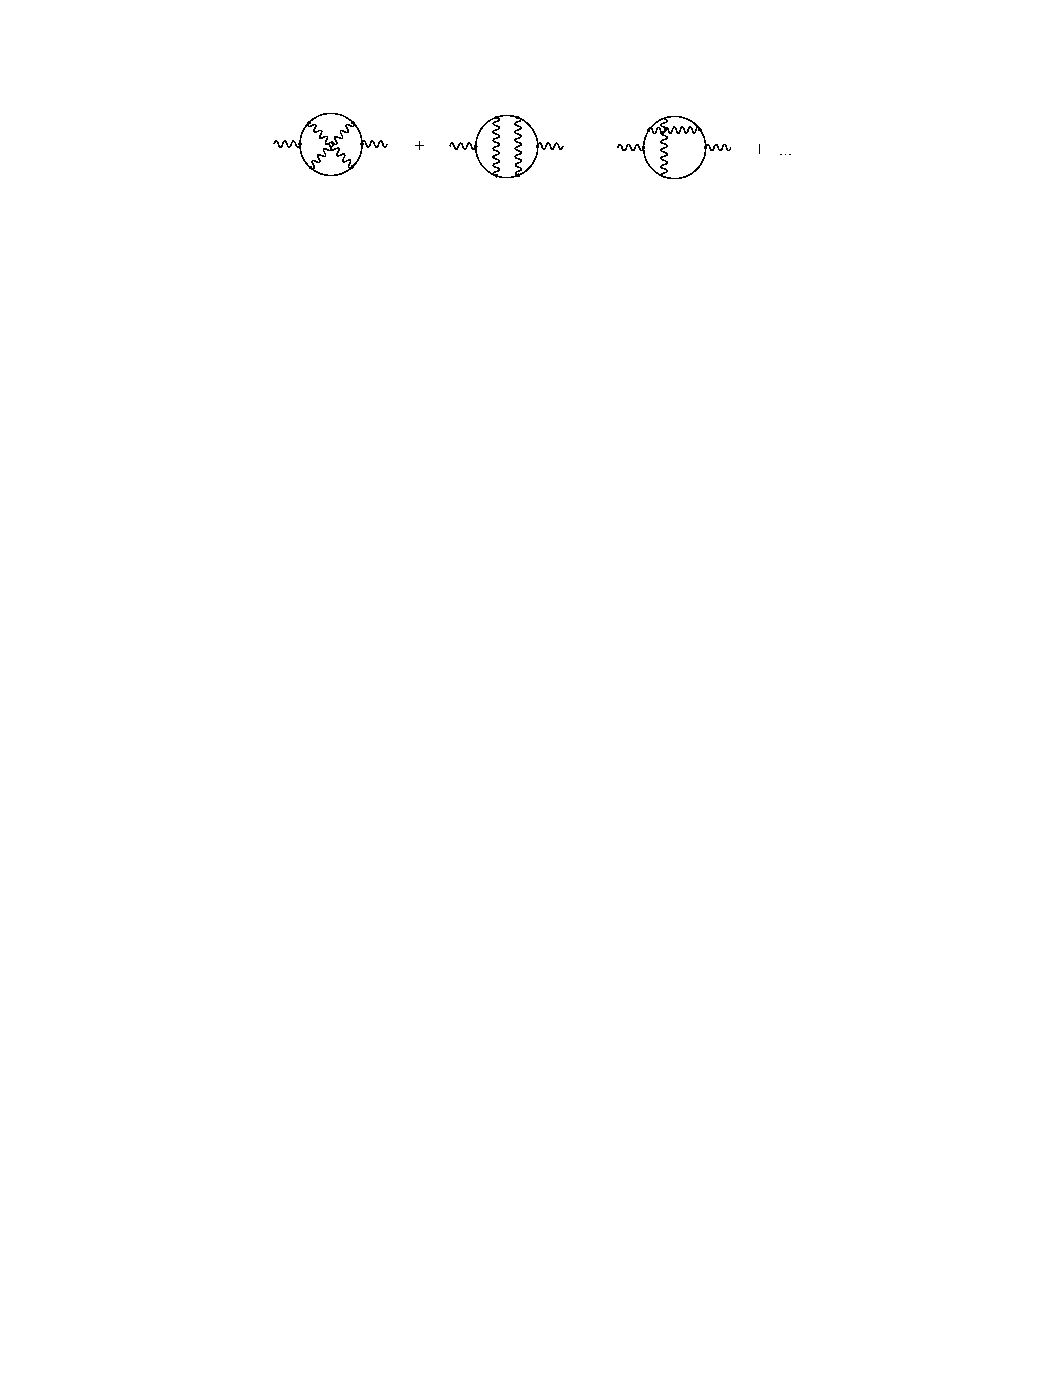
\includegraphics[width=1\textwidth]{BHSTW143loopphotonprop}
 \caption{
 Quenched diagrams contributing to the three loop QED photon propagator.
 From \refref{BHSTW14}.
 }
 \label{BHSTW143loopphotonprop}
\end{figure}
%%%%%%%%%%%%%%%%%%%%%%%%%%%%%%%%%%%%%%%%%%%%%%%%%

Thus, for the quenched scalar QED, the worldline integrals are expressed
in terms of $N$-photon propagators, the central ingredient that defines
the quenched gauge sets \refeq{quenchAnom}.
Unlike the Feynman parameter integrals for individual vertex graphs, they are
independent of the ordering of the momenta $k_1,\ldots,k_N$; the formula
\refeq{AhBaSc16(1)i} contains all $\approx N!$ ways of attaching the $N$
photons to the charged particle propagator.
The formulation combines combinatorially many Feynman diagrams into a single integral.
An example are the quenched contributions to the
three-loop photon propagator shown in \reffig{BHSTW143loopphotonprop}.

In QED the $N$-photon propagator formulation combines into one integral
all Feynman graphs related by permutations of photon legs along fermion
lines, that is, it should yield \emph{one} integral for a gauge set
$km'm$ defined in \refeq{quenchAnom}.
%, provided one may distinguish the leg-photons from the cross-photons.

\subsection{High-orders QED in worldline formalism}
\label{sect:highQEDworldline}

A non-perturbative formula for QED in a constant field, given for scalar
QED in 1982 by Affleck, Alvarez, and Manton\rf{AffAlMa82} is an example how the
worldline formalism can yield high-order information on QED amplitudes.
Huet, McKeon, and Schubert\rf{HuMcSc10} continue this in their 2010
%{\em {Euler-Heisenberg} lagrangians and asymptotic analysis in 1+1 {QED.
% Part I: Two}-loop}
%(no GaTech online access, \arXiv{1010.5315}):``
study of the l-electron loop, $N$-photon amplitudes in the limit of large
photon numbers and low photon energies, this time for 1+1 dimensional
scalar QED, in order to illustrate the large cancellations inside gauge
invariant classes of graphs.

Affleck \etal\rf{AffAlMa82} use the Feynman\rf{Feynman50} `worldline
path integral' representation of the quenched effective action for scalar
QED in the constant electric field, and calculate the amplitude in a
stationary path approximation. The stationary trajectory so obtained is a
circle with a field dependent radius, called ``instanton''  in this
context. The worldline action on this trajectory yields the correct
exponent, and the second variation determinant yields the correct  prefactor.
Using Borel analysis, they obtain non-perturbative information on the
on-shell renormalized $N$-photon amplitudes at large $N$ and low energies.

Parenthetically, independently and not by worldline formalism, but by
dint of difficult calculations and much deep physics intuition, Lebedev
and Ritus\rf{LebRit84} have arrived at a nonperturbative mass shift
interpretation for the spinor QED pair creation in constant electric
field in 1984.

For the quenched spinor QED (fermion lines decorated by photon exchanges)
closed-form expressions for general $N$ require the worldline
super-\,formalism\rf{Schubert01}, at the cost of introducing Fradkin
1966\rf{Fradkin66} Grassmann path integral,
or, alternatively,
the second order
formalism of Strassler\rf{Strassler92}.


% \item[2017-07-05 Christian] read
The  2017 G. Torgrimsson, Schneider,  Oertel and Schützhold\rf{TSOS17},
% {\em Dynamically assisted {Sauter-Schwinger} effect - non-perturbative
% versus perturbative aspects},
\arXiv{1703.09203}, sect.~3,
uses the $N$-photon formalism to determine a saddle and the asymptotic
form of two types of dynamically assisted {Sauter-Schwinger} effect.

The 2006 Dunne and Schubert\rf{DunSch06} study of scalar and spinor QED
$N$-photon amplitudes, in the quenched approximation (\ie, taking only
the diagrams with one electron loop) led to ``the following
generalization of Cvitanovi\'c's conjecture: the perturbation series
converges for all on-shell renormalized QED amplitudes at leading order
in $N_f$. It must be emphasized that the on-shell renormalization is
essential in all of the above.''
Unlike Cvitanovi\'c\rf{Cvit77b} purely numerical conjecture, theirs is a
sophisticated argument, buttressed by Borel dispersion relations.


\subsection{Electron magnetic moment in worldline formalism}
\label{sect:magMomWorldline}

Here we specialize the electron magnetic moment discussion of
\refsect{sect:magMom} to the quenched subsector.
$Z_1$,
$Z_2$, and % = (1-B)^{-1}$, and
$Z_3$,
are the respectively the vertex,
the electron wave function, and
the photon wave function
renormalization constants.
For quenched QED there are no
fermion loops, there are no vacuum polarization contribution to the charge
renormalization \refeq{IRstruct(3)}, $Z=Z_3=1$, so the bare coupling equals
the physical coupling, $\alpha_0= \alpha$.
Furthermore, $Z_1=Z_2$ by the Ward identity\rf{Ward50}.


%%%%%%%%%%%%%%% start inseert %%%%%%%%%%%%%%%%%%%%%%%%%%%%
%\section{Electron magnetic moment}
The anomalous magnetic moment of an electron $a = (g-2)/2$ is
given by the static limit of the magnetic form factor
$a=\tilde{F}_2(0)=M/(1+L)$ from \refeq{PRD10-74-III(2.2)},
with perturbative expansion
\beq
a = \frac{M(\alpha)}{1+L(\alpha)}
  =  \sum_{n=1}^\infty
          a^{(2n)}\left(\frac{\alpha}{\pi}\right)^{n}
\,,
\ee{IRstruct(1)Q}
where $Z_1=1+L =F_1(0)$, $M=F_2(0)$ are computed from the unrenormalized
on-shell values of proper vertex \refeq{BAGTB17(35-1)}, given by the sum
of all one-particle irreducible (1pI) electron-electron-photon vertex
diagrams with internal photon corrections (no electron loops).
Expanding $M$ and $L$ we have
\bea
a_{0}^{(2)} &=& M^{(2)}
            \continue
a_{0}^{(4)} &=& M^{(4)} - L^{(2)}M^{(2)}
            \label{PRD10-74-III(2.6)Q}\\
a_{0}^{(6)} &=& M^{(6)} - L^{(2)}M^{(4)} - (L^{(4)} - (L^{(2)})^2) M^{(2)}
\nnu
\eea
Each order in
\refeq{IRstruct(1)Q} is IR and UV finite, with the UV subdivergences are
cancelled by $L^{(2m)}$ counterterms in \refeq{PRD10-74-III(2.6)Q}.

A gauge set $km'm$ in expansion \refeq{quenchAnom} consists of all 1-particle irreducible vertex
diagrams without electron loops, with $k$ photons crossing the external
vertex (cross-photons) and $m [m']$ photons originating and terminating
on the incoming [outgoing] electron leg (leg-photons). One can assume
three different coupling, setting them all equal to $\alpha$ at the
end of the calculation,
\beq
a =
          \sum_{m'=0}^\infty\left(\frac{\alpha'}{\pi}\right)^{m'}
          \sum_{k=1}^\infty\left(\frac{\alpha_v}{\pi}\right)^{k}
          \sum_{m=0}^\infty\left(\frac{\alpha}{\pi}\right)^{m}
          a_{km'm}
\,.
\ee{quenchAnomQ}
The gauge set contributions are then
\bea
a^{(2)} &=& a_{100}
            \continue
a^{(4)} &=& a_{200} + a_{110} + a_{101}
            \label{gaugeSets}\\
a^{(6)} &=&  a_{300} + a_{210} + a_{201} +  a_{120} + a_{102} + a_{111}
            \continue
a^{(8)} &=& a_{400} + a_{310} + a_{301}  +  a_{220} + a_{202} + a_{211}
         +  a_{130} + a_{103} + a_{121} + a_{112}
            \continue
a^{(10)}&=& a_{500} + a_{410} + a_{401} +  a_{320} + a_{302} + a_{311}
         +  a_{230} + a_{203} + a_{221} + a_{212}
            \ceq
         +  a_{140} + a_{104} + a_{131} + a_{113} + a_{122}
\nnu
\eea




Both $L^{(2m)}$ and $M^{(2m)}$ can be evaluated in terms of
$N$-photon propagators.

\begin{enumerate}
  \item
To proceed, one needs something like a Bern-Kosower\rf{BerKos91} type
master formula for the electron line dressed with any number of photons,
with a single constant external (arbitrarily weak) magnetic field insertion.
% Schubert \etal\ have it (unpublished).
For the magnetic moment calculation, the external vertex is distinguished
by its
\(
\sigma^{\mu\nu}={1\over 2}[\gamma^{\mu},\gamma^{\nu}]
\)
form \refeq{BAGTB17(35-1)}, while all internal, virtual photon vertices
are of the usual $\gamma^{\mu}$ form.
  \item
Please write down
the worldline formula for the anomalous magnetic moment
of the electron $a=\tilde{F}_2(0)$, corresponding to Dirac trace
expression \refeq{PRD10-74-III(2.2)} for $M$.
  \item
As the external vertex transfers a (vanishing) momentum, the
incoming and outgoing electron on-mass shell legs are distinct, and thus
there are three kinds of $N$-photon propagators; $k$ photons crossing the
external vertex (cross-photons) and $m [m']$ photons originating and
terminating on the incoming [outgoing] electron leg (leg-photons). One
needs to prove in the worldline formalism that each $km'm$
integral (corresponding to a set of quenched set of 1-particle
irreducible Feynman vertex diagrams without electron loops) is separately
(i) a gauge set, and
(ii) the minimal gauge invariant set.
  \item
Hopefully the distinction motivates the  gauge set sign rule
\refeq{Cvit77b(5)}. Keep in mind, however, that this empirical rule is
already violated by the gauge set $(2,2,0)$.
  \item
Please write down
the worldline integral for one-loop anomaly $a_{0}^{(2)}$ in
\refeq{PRD10-74-III(2.6)}.
The first thing to verify is that the worldline $(1,0,0)$ integral
reproduces Schwinger's $\frac{1}{2}\left(\frac{\alpha}{\pi}\right)$
result\rf{Schwinger48}, exactly. That is an exercise in converting the
integral into Feynman-parametric form, already done several times for
other amplitudes.
  \item
Please write down the worldline integral for 2-loop anomaly
$a_{0}^{(4)}=M^{(4)}-L^{(2)}M^{(2)}$ in \refeq{PRD10-74-III(2.6)}.
Can $L^{(2)}M^{(2)}$ be absorbed into the integrand? If cancelations can
be made pointwise, that would obviate a need for constructing UV  (and
IR?) counterterms.
  \item
For 2-loop anomaly there are only 2 quenched gauge sets $km'm$:
$(2,0,0)$ and $(1,1,0)$, which equals $(1,0,1)$ by time reversal, see
\reffig{Cvit77bFig1} and \reftab{tabGaugeSets}.
So, reformulate the 2-loop calculation as two worldline integrals,
one for each gauge set.
Most likely, want to do the gauge set $(2,0,0)$ first, as it seems to
have simpler subdiagram structure (though not sure about that).
Do not attempt (for now) to evaluate these analytically (though
Broadhurst, Laporta,
Kreimer, \etc, would be interested to see whether some simplification
occurs), main thing is to understand that the UV renormalization works,
and that there are no intermediate IR divergences in this reformulation.
\end{enumerate}
